\chapter{Supplementary Results} % Main appendix title
\label{app:suppresults}
\section{Semantic Embeddings}
\subsection{Visualization of Semantic Spaces with TensorFlow Projector}
[TODO: analysis of general form, examples by listing the most close words in space]

\begin{figure}
    \centering
    \begin{minipage}[t]{.5\textwidth}
        \centering
        \makebox[.5\linewidth]{
        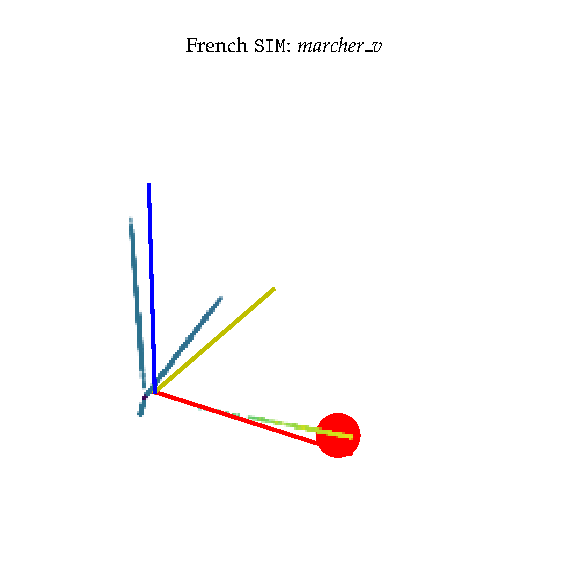
\includegraphics[scale=1]{Figures/FreSIMPCAformarcher_v.pdf}
        }
        \caption[French \code{SIM} Space Visualization]{Due to the nature of WOLF, 
        \code{SIM}'s first PCs denotes POS category. Light colors indicate the proximity of the represented words with \emph{marcher\_v}.}
        \label{fig:freSIMmarcher}
    \end{minipage}%
    \begin{minipage}[t]{.5\textwidth}
        \centering
        \makebox[.5\linewidth]{
        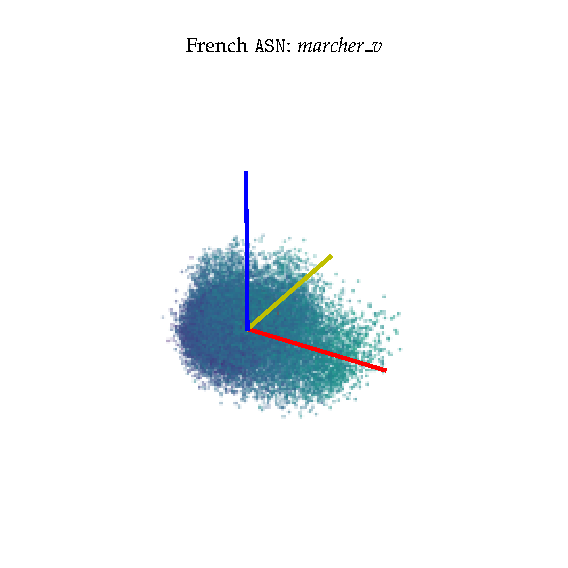
\includegraphics[scale=1]{Figures/FreASNPCAformarcher_v.pdf}
        }
        \caption[French \code{ASN} Space Visualization]{\code{ASN}'s variance are more homogeneously distributed over PCs.}
        \label{fig:freASNmarcher}
    \end{minipage}
\end{figure}


\begin{figure}
    \centering
    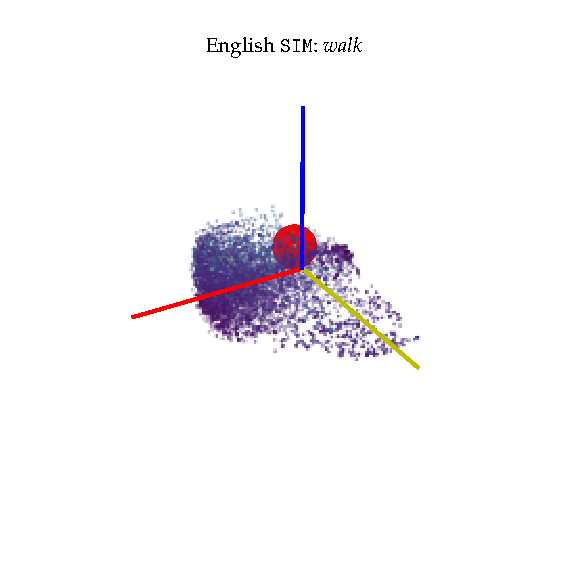
\includegraphics[scale=1]{Figures/EngSIMPCAforwalk.pdf}
    \caption[English \code{SIM} Space Visualization]{English's \code{SIM} however seems not to be macroscopically influenced by POS information.}
    \label{fig:engSIMwalk}
\end{figure}

\label{appsubsec:projectorvisu}
\subsection{Semantic Ranking Task Results}
\label{appsubsec:wnembeddingtests}
% \subsection{English \code{WordNetEmbedding} Iterations}
\begin{table}
\begin{tabularx}{\textwidth}{*{9}{X}}
    \toprule
    {} &                                         Unnamed: 1 &                                   Unnamed: 2 & Unnamed: 3 & Unnamed: 4 & Similarity & Unnamed: 6 & Unnamed: 7 & Association \\
    \midrule
    0  &                                          Relations &                              Vocabulary Size &  Dimension &     Metric &     SIMLEX &  WS353-SIM &     RG1965 &   WS353-ASN \\
    1  &                                                NaN &                                          NaN &        NaN &        OOV &      0.002 &       0.02 &          0 &       0.012 \\
    2  &                                           Synonymy &                                          15k &        850 &    Pearson &     0.2256 &     0.2679 &     0.3627 &       0.123 \\
    3  &                                                NaN &                                          NaN &        NaN &   Spearman &     0.2001 &     0.2003 &     0.3403 &      0.0971 \\
    4  &                                           Synonymy &                                          60k &        850 &    Pearson &      0.234 &     0.2112 &     0.3394 &      0.1449 \\
    5  &                                                NaN &                                          NaN &        NaN &   Spearman &     0.1747 &     0.1895 &     0.2629 &      0.1129 \\
    6  &                                     Syn + Antonymy &                                          15k &        850 &    Pearson &     0.1534 &     0.2743 &      0.373 &      0.0969 \\
    7  &                                                NaN &                                          NaN &        NaN &   Spearman &     0.1255 &     0.1922 &     0.3302 &      0.0817 \\
    8  &                         Syn + Hypernymy + Hyponymy &                                          15k &        850 &    Pearson &     0.3904 &     0.4825 &     0.6187 &      0.0373 \\
    9  &                                                NaN &                                          NaN &        NaN &   Spearman &     0.4018 &     0.3856 &     0.5145 &      0.0259 \\
    10 &  Syn + Hyper+ Hypo + adj.participle\_of\_verb + a... &                                          15k &        850 &    Pearson &     0.5079 &     0.5333 &     0.6784 &      0.0525 \\
    11 &                                                NaN &                                          NaN &        NaN &   Spearman &     0.4986 &     0.4214 &      0.576 &      0.0272 \\
    12 &  Syn + hyper + hypo + participle + adj.similar ... &                                          15k &        511 &    Pearson &      0.506 &        NaN &        NaN &      0.0279 \\
    13 &                                                NaN &                                          NaN &        NaN &   Spearman &     0.4989 &        NaN &        NaN &      0.0193 \\
    14 &  Syn + hyper + hypo + participle + adj.similar ... &                                          60k &        511 &    Pearson &     0.5268 &     0.5483 &     0.6991 &      0.1092 \\
    15 &                                                NaN &                                          NaN &        NaN &   Spearman &     0.5152 &     0.4757 &     0.5501 &      0.0515 \\
    16 &                                                NaN &                                          NaN &        NaN &        NaN &        NaN &        NaN &        NaN &         NaN \\
    17 &                                      Common Crawl  &                                  2.2M, cased &        300 &    Pearson &     0.3946 &     0.6573 &     0.6812 &      0.6091 \\
    18 &                                                NaN &                                          NaN &        NaN &   Spearman &     0.3752 &     0.6298 &     0.6577 &      0.5709 \\
    19 &                                                NaN &                                          NaN &        NaN &        OOV &        0.1 &          0 &          0 &           0 \\
    20 &                             CommonCraw - 01-23 Sim &                                         8157 &        300 &    Pearson &     0.1953 &     0.5854 &     0.5547 &      0.5633 \\
    21 &                                                NaN &                                          NaN &        NaN &   Spearman &     0.2133 &     0.5719 &     0.5641 &      0.5918 \\
    22 &                                                NaN &                                          NaN &        NaN &        OOV &        NaN &        NaN &        NaN &         NaN \\
    23 &                                                All &                                 13k specific &        850 &    Pearson &        0.5 &       0.65 &       0.65 &        0.32 \\
    24 &                                                NaN &                                          NaN &        NaN &   Spearman &       0.52 &       0.67 &       0.75 &        0.33 \\
    25 &                                                NaN &                                   60k random &        NaN &    Pearson &        0.5 &       0.51 &       0.56 &        0.31 \\
    26 &                                                NaN &                                          NaN &        NaN &   Spearman &       0.51 &       0.58 &       0.72 &         0.3 \\
    27 &                                   Synonym Database &  60k (multi-word phrases eliminated → 36718) &        850 &    Pearson &     0.6814 &     0.5819 &     0.8155 &       0.317 \\
    28 &                                                NaN &                                          NaN &        NaN &   Spearman &     0.6566 &     0.4677 &     0.7032 &      0.3153 \\
    29 &                                                NaN &                                          NaN &        NaN &        OOV &        6.6 &       22.7 &        7.7 &          19 \\
    \bottomrule
    \end{tabularx}
\end{table}

\subsection{Vocabulary Coverage by POS}
\begin{table}
    \centering
    \begin{ThreePartTable}
        
    \begin{tabularx}{\textwidth}{L *{10}{R}}
    \multicolumn{11}{l}{\tabhead{The Little Prince Vocabulary Coverage}} \\
    \toprule
    &  & \multicolumn{9}{l}{\tabhead{\# Instances in fMRI Recording Session}} \\
    \toprule
    \mr{2}{*}{Story} & \textbf{T} & 725 & 812 & 860 & 762 & 732 & 902 & 819 & 712 & 802 \\
    & \textbf{V} & F & 812 & 860 & 762 & 732 & 902 & 819 & 712 & 802 \\
    \midrule
    \mr{4}{*}{\parbox{0.8cm}{\code{SIM} 56665}} & TM & 36 & 30 & 32 & 27 & 30 & 33 & 24 & 30 & 27 \\
    & \% & F & 812 & 860 & 762 & 732 & 902 & 819 & 712 & 802 \\
    & VM & F & 812 & 860 & 762 & 732 & 902 & 819 & 712 & 802 \\
    & \% & F & 812 & 860 & 762 & 732 & 902 & 819 & 712 & 802 \\
    \midrule
    \mr{4}{*}{\parbox{0.8cm}{\code{ASN} /\code{MIX} /\code{SIG} 24519}} & TM & 48 & 47 & 38 & 37 & 48 & 60 & 35  & 37 & 41 \\
    & \% & F & 812 & 860 & 762 & 732 & 902 & 819 & 712 & 802 \\
    & VM & F & 812 & 860 & 762 & 732 & 902 & 819 & 712 & 802 \\
    & \% & F & 812 & 860 & 762 & 732 & 902 & 819 & 712 & 802 \\
    \bottomrule
    \end{tabularx}
    \end{ThreePartTable}
    \caption[The Little Prince Vocabulary Coverage in Semantic Spaces]{\textbf{T}: Token, \textbf{V}: Vocabulary, M: Miss\label{apptab:lppcoverage}}
    \end{table}

\subsection{Corpus-Targeted Semantic Feature Selection}
\begin{figure}
    \centering
    \makebox[\linewidth]{
    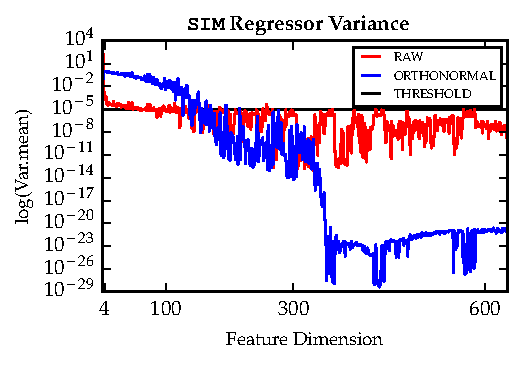
\includegraphics[scale=1]{Figures/SimDimensionSelectionRegLPP.pdf}
    }
    \caption[French \code{MIX} Regressor Variances]{Placeholder} 
    \label{fig:freMIXRegVar}
\end{figure}
\begin{figure}
    \centering
    \makebox[\linewidth]{
    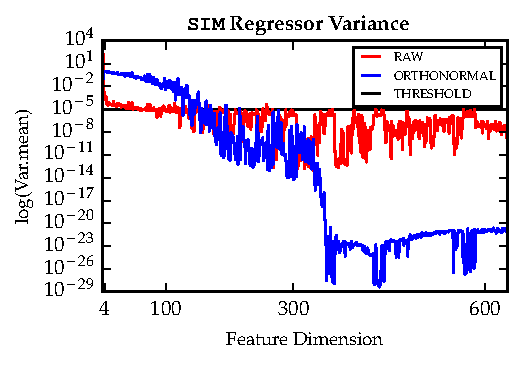
\includegraphics[scale=1]{Figures/SimDimensionSelectionRegLPP.pdf}
    }
    \caption[French \code{SIG} Regressor Variances]{Placeholder} 
    \label{fig:freSIGRegVar}
\end{figure}


\section{Non-nested Model Comparison}
\label{appsubsec:nonnestedcompres}

\section{Regression}
\subsection{More on \(\alpha\) and Dimension Selection}
\label{appsubsec:alphadim}
[TODO, alpha and dim values]

[TODO: histogram animation with alpha evolution, ]

[TODO: discussion on overfit by dimension, despite regularization]